\documentclass[11pt,]{article}
\usepackage{lmodern}
\usepackage{amssymb,amsmath}
\usepackage{ifxetex,ifluatex}
\usepackage{fixltx2e} % provides \textsubscript
\ifnum 0\ifxetex 1\fi\ifluatex 1\fi=0 % if pdftex
  \usepackage[T1]{fontenc}
  \usepackage[utf8]{inputenc}
\else % if luatex or xelatex
  \ifxetex
    \usepackage{mathspec}
  \else
    \usepackage{fontspec}
  \fi
  \defaultfontfeatures{Ligatures=TeX,Scale=MatchLowercase}
\fi
% use upquote if available, for straight quotes in verbatim environments
\IfFileExists{upquote.sty}{\usepackage{upquote}}{}
% use microtype if available
\IfFileExists{microtype.sty}{%
\usepackage{microtype}
\UseMicrotypeSet[protrusion]{basicmath} % disable protrusion for tt fonts
}{}
\usepackage[margin=1in]{geometry}
\usepackage{hyperref}
\hypersetup{unicode=true,
            pdfborder={0 0 0},
            breaklinks=true}
\urlstyle{same}  % don't use monospace font for urls
\usepackage{graphicx,grffile}
\makeatletter
\def\maxwidth{\ifdim\Gin@nat@width>\linewidth\linewidth\else\Gin@nat@width\fi}
\def\maxheight{\ifdim\Gin@nat@height>\textheight\textheight\else\Gin@nat@height\fi}
\makeatother
% Scale images if necessary, so that they will not overflow the page
% margins by default, and it is still possible to overwrite the defaults
% using explicit options in \includegraphics[width, height, ...]{}
\setkeys{Gin}{width=\maxwidth,height=\maxheight,keepaspectratio}
\IfFileExists{parskip.sty}{%
\usepackage{parskip}
}{% else
\setlength{\parindent}{0pt}
\setlength{\parskip}{6pt plus 2pt minus 1pt}
}
\setlength{\emergencystretch}{3em}  % prevent overfull lines
\providecommand{\tightlist}{%
  \setlength{\itemsep}{0pt}\setlength{\parskip}{0pt}}
\setcounter{secnumdepth}{0}
% Redefines (sub)paragraphs to behave more like sections
\ifx\paragraph\undefined\else
\let\oldparagraph\paragraph
\renewcommand{\paragraph}[1]{\oldparagraph{#1}\mbox{}}
\fi
\ifx\subparagraph\undefined\else
\let\oldsubparagraph\subparagraph
\renewcommand{\subparagraph}[1]{\oldsubparagraph{#1}\mbox{}}
\fi

%%% Use protect on footnotes to avoid problems with footnotes in titles
\let\rmarkdownfootnote\footnote%
\def\footnote{\protect\rmarkdownfootnote}

%%% Change title format to be more compact
\usepackage{titling}

% Create subtitle command for use in maketitle
\providecommand{\subtitle}[1]{
  \posttitle{
    \begin{center}\large#1\end{center}
    }
}

\setlength{\droptitle}{-2em}

  \title{}
    \pretitle{\vspace{\droptitle}}
  \posttitle{}
    \author{}
    \preauthor{}\postauthor{}
    \date{}
    \predate{}\postdate{}
  
\usepackage{booktabs}
\usepackage{longtable}
\usepackage{array}
\usepackage{multirow}
\usepackage{wrapfig}
\usepackage{float}
\usepackage{colortbl}
\usepackage{pdflscape}
\usepackage{tabu}
\usepackage{threeparttable}
\usepackage{threeparttablex}
\usepackage[normalem]{ulem}
\usepackage{makecell}
\usepackage{xcolor}

\usepackage[natbibapa, sectionbib, tocbib]{apacite}
\usepackage[utf8]{inputenc}
\usepackage[singlelinecheck = off]{caption}
\usepackage{lmodern}
\usepackage{microtype}
\usepackage{multirow}
\usepackage[inline]{enumitem}
\usepackage{array}
\usepackage[htt]{hyphenat}
\usepackage{booktabs}
\usepackage[euler]{textgreek}
\usepackage{float}
\usepackage[doublespacing]{setspace}
\usepackage{fancyhdr}
\captionsetup[table]{width=\textwidth}
\setlength{\parindent}{2em}
\fancyhf{}
\fancyhead[RH]{\thepage}
\renewcommand{\headrulewidth}{0pt}
\pagestyle{fancy}
\hypersetup{colorlinks = true, linkcolor = blue, urlcolor = black, citecolor = blue}
\DeclareCaptionFormat{apa}{#1#2\\[1em]#3}
\captionsetup*[table]{labelsep = none, textfont = it, format = apa, width = .8\textwidth}
\captionsetup*[figure]{labelsep = period, labelfont = it, position = below, skip = -10pt}

\begin{document}

\hypertarget{participants}{%
\subsection{Participants}\label{participants}}

Undergraduate and graduate phonetics and psychology students (80.8\%
female, median age = 21, IQR = 3, range = {[}18, 31{]}, total \(N\) =
207) participated in the study in exchange for course credit.
Participants were randomly assigned to one of five groups which differed
in the type of activity they engaged in between parts of the text they
have read and in whether they received feedback on their intermittent
test achievement or not.

\hypertarget{materials-and-procedure}{%
\subsection{Materials and procedure}\label{materials-and-procedure}}

\hypertarget{materials}{%
\subsubsection{Materials}\label{materials}}

Participants read a text on the evolution, ecological and biological
characteristics of weeds. The text was taken from a chapter in a
university-level textbook. Some sentences and passages were slightly
modified, so as to avoid odd language constructions; Latin plant names
were translated, and some plants were removed from the text to make it
less difficult for the target participant population. The text was
divided into three parts of 874, 754, and 835 words, respectively.
Additionally, there was a practice text taken from the same chapter, but
unrelated to any of the other three parts of the text (768 words). The
materials were presented on a personal computer, in an application
constructed using the open source \textit{oTree} framework
\citep[version 2.1.35,][]{chenOTreeOpensourcePlatform2016} for the
\textit{Python} programming language (version 3.6.4, October 20, 2018).

\hypertarget{procedure}{%
\subsubsection{Procedure}\label{procedure}}

We have manipulated two aspects of the experimental procedure, which we
will describe in turn. The first aspect is the interpolated activity
that the participants engaged in between parts of the text. Participants
either (i) answered ten questions related to the content of the part
they have previously read, (ii) answered ten general knowledge questions
or (iii) reread the same part of the text they have previously read.

The second aspect we have manipulated is whether or not participants
received feedback on their accomplishment on the interpolated tests.
Obviously, this manipulation applies only to the participants in the
general-knowledge and content-related testing conditions, which means
that there were five experimental conditions. Feedback was presented on
a separate screen which listed the questions, the participant's answers,
and the correct answers in a tabular format. Incorrectly answered
questions were highlighted in red, and correctly answered questions in
green. After 40 seconds elapsed, a ``Next'' button appeared, allowing
participants to proceed to the next text. By setting this cooldown
period, by emphasising that there would be a cumulative test, and
through written instructions, we wanted to encourage our participants to
carefully examine the feedback. The feedback was presented for maximally
60 seconds, after which the application proceeded to the next text.

\begin{figure}
  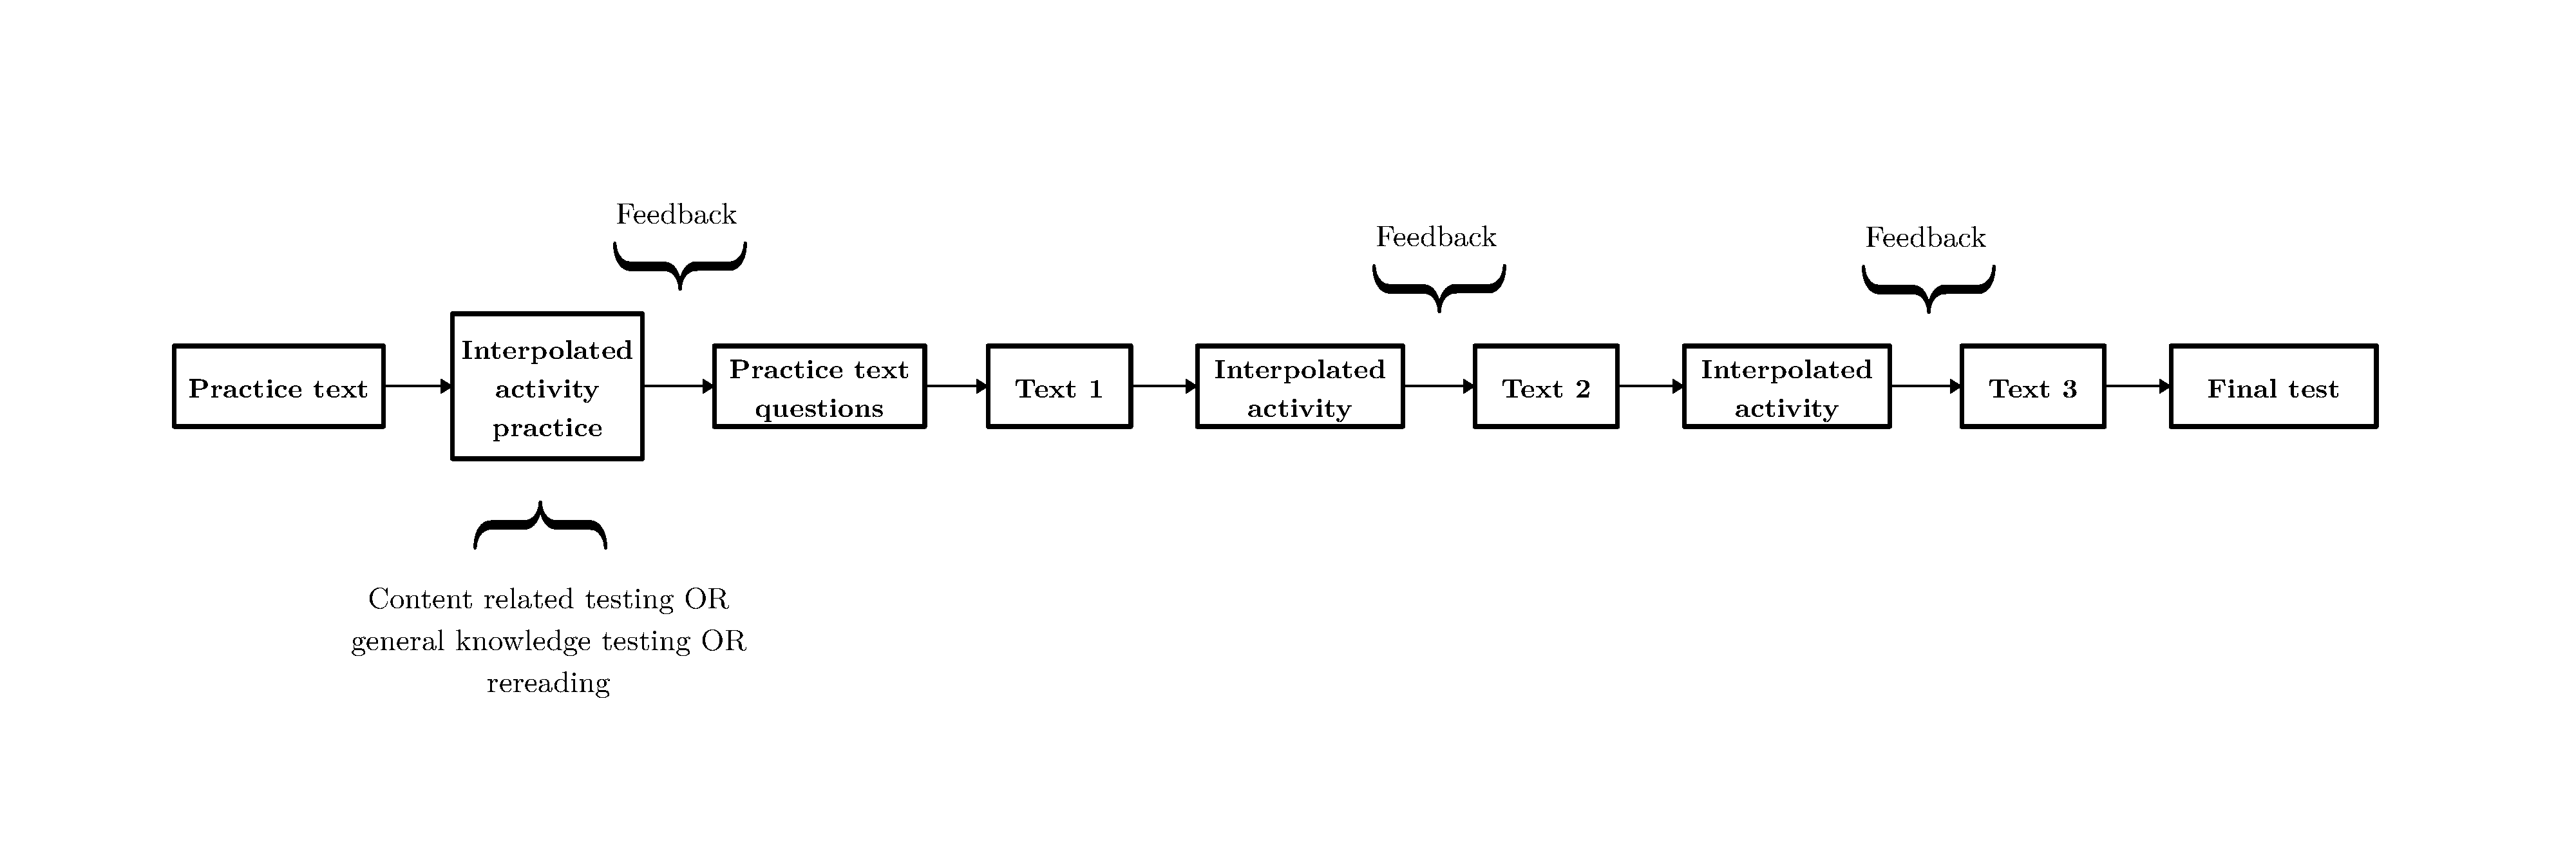
\includegraphics[width = \textwidth, keepaspectratio, trim = 135 0 135 90]{../images/flowchart/procedure.pdf}
  \caption{A flowchart depicting the experimental procedure.}
  \label{flowchart}
\end{figure}

We will now describe the general procedure. Participants were first
given a brief introduction to the study, and were encouraged to
carefully read and follow the written instructions. Then, they were led
to a computer which was running a fullscreen instance of the
\textit{oTree} application with a randomly chosen experimental
condition. There, participants read the informed consent form and, in
case there were no questions, started the experiment. A flowchart for
the experiment is displayed in Figure \ref{flowchart}.

After entering their personal information, participants were presented
with the instructions for their first task, which was to read the
practice text at a speed that comes naturally to them. They were to
click a button at the bottom of the text when they have finished reading
it. Unbeknownst to the participants, the time they took to read the
practice text was recorded, and used as the basis for determining the
reading time limits for the remaining texts. However, the lowest
possible time limit was set to 5 minutes, and the longest to 8 minutes.

Next, participants were familiarised with the interpolated activity they
were going to perform during the main part of the procedure. The
content-related test group answered four questions based on the practice
text, the general-knowledge test group answered four general knowledge
questions, and the rereading group reread the practice text (this time
with the time limit applied). Subjects in the rereading and general
knowledge conditions also answered the four questions related to the
practice text, in order to familiarise themselves with the scope and
specificity level of the questions they will receive after reading the
final text. Participants assigned to the feedback condition also
received feedback on their interpolated activity practice test
achievement.

After the practice round, participants proceeded to the main part of the
study, engaging in the interpolated activities they were assigned.
Depending on the condition they were assigned to, they also received
feedback after every interpolated test.

All participants were told that there would be a cumulative test after
the final part of the text, examining their knowledge of all three
parts. In reality, the final test examined only the knowledge of the
final part. Participants were presented with twenty questions examining
their knowledge of that part. No feedback was presented after the final
test, irrespective of the experimental condition. The computer recorded
whether a participant correctly answered a question and whether the
participant chose an intrusive distractor. This allowed us to compute
our dependent variables --- the total number of correct answers and the
total number of intrusive distractors chosen. We will now describe the
test questions.

In total, forty-four content related questions with four response
options were generated from the presented parts of the text. Four
questions were presented after the practice text, ten after each of the
first two parts (only to the participants in the content related test
condition), and twenty after the third part of the text (to all
participants). Starting from the second ten-question-set, the distractor
options were chosen so that (a) two distractors were plausible, but
unrelated to the text, and (b) one distractor was a term or concept
mentioned in the previous part of the text --- this was considered to be
the ``intrusive'' distractor (sometimes reffered to as the ``intrusor''
in the rest of this article). Further, twenty-four general knowledge
questions were generated. These questions were presented to participants
in the general-knowledge test condition, after the first two parts of
the text and after the practice text.

\hypertarget{results}{%
\subsection{Results}\label{results}}

\hypertarget{exclusion-criteria}{%
\subsubsection{Exclusion criteria}\label{exclusion-criteria}}

\begin{table*}[t]

\caption{\label{tab:descTable}\label{descTable}Descriptive statistics for the DVs broken down
                     by experimental condition.}
\centering
\begin{tabular}{llrrrrrr}
\toprule
Measure & Condition & $n$ & $M$ & $SE_M$ & $SD$ & min & max\\
\midrule
 & Content, feedback & 41 & 13.22 & 0.508 & 3.25 & 2 & 19\\

 & Content, no feedback & 42 & 12.79 & 0.465 & 3.02 & 7 & 19\\

 & General, feedback & 40 & 10.97 & 0.533 & 3.37 & 1 & 17\\

 & General, no feedback & 40 & 10.47 & 0.449 & 2.84 & 5 & 16\\

\multirow{-5}{*}{\raggedright\arraybackslash Total correct} & Rereading & 40 & 10.88 & 0.443 & 2.80 & 4 & 17\\
\cmidrule{1-8}
 & Content, feedback & 41 & 3.15 & 0.258 & 1.65 & 0 & 7\\

 & Content, no feedback & 42 & 3.38 & 0.257 & 1.67 & 0 & 7\\

 & General, feedback & 40 & 4.17 & 0.318 & 2.01 & 0 & 8\\

 & General, no feedback & 40 & 4.58 & 0.288 & 1.82 & 1 & 9\\

\multirow{-5}{*}{\raggedright\arraybackslash Total intrusors} & Rereading & 40 & 4.62 & 0.350 & 2.21 & 1 & 10\\
\bottomrule
\end{tabular}
\end{table*}

Prior to analysing the data, we have excluded participants based on a
priori set criteria. Participants who have spent less than or equal to
90 seconds on the practice text were excluded (1 exclusion). Further, we
wanted to exclude participants who have had no correct answers on the
final test (0 exclusions). Finally, we have excluded participants who
have stated that they have reading deficits (3 exclusions). This left us
with a total sample of 203 participants. The descriptives for the sample
are shown in Table \ref{descTable}. There is another set of exclusion
criteria based on the number of times the participants have read each of
the three texts. These are used in robustness check analyses (see
supplementary materials).

\hypertarget{interpolated-activity-effect}{%
\subsubsection{Interpolated activity
effect}\label{interpolated-activity-effect}}

Our first two hypotheses are concerned with the effects of different
interpolated activities on the total number of correct answers and total
number of intrusive distractors chosen. To test these hypotheses, we
have focused only on the groups which have not received feedback (\(n\)
= 122). This was done because there was no feedback option for the
rereading group, and we did not want to treat the feedback and
no-feedback general-knowledge and content-related testing groups as
equivalent without strong evidence supporting that assumption. We
conducted a one-way MANOVA with interpolated activity as the independent
variable and the total number of correct and intrusive options chosen as
dependent variables. The correlation between our DVs calculated on the
whole sample is \(r =\) -.707 (95\% CI: {[}-.77, -.63{]}, \(p\)
\textless{} .0001).

Pillai's V for the analysis is .126, \(p = .004\) (Wilks' \(\Lambda\) =
.875, \(p = .003\)). The effect size, calculated as
\(\omega^2_{mult} = .109\) (bootstrap
median\footnote{All bootstrap estimates taken from 10000 replications.}
= .132, \(BC_\alpha\) 95\% CI = {[}.012, .201{]}). To further inspect
the relationship of the interpolated activities with our dependent
variables, we have conducted a Roy-Bargmann stepdown analysis, as
suggested by \citeauthor{tabachnickUsingMultivariateStatistics2012}
(\citeyear{tabachnickUsingMultivariateStatistics2012}; a linear
discriminant analysis with the same aim is available in the
supplementary materials). The total number of correct answers was a
priori chosen to be the higher priority variable. According to
\citet{tabachnickUsingMultivariateStatistics2012}, the higher priority
variable can be chosen based on theoretical or practical grounds. Since,
the total number of correct answers is the criterion that determines a
student's success in a testing context, we have chosen this dependent
variable as the higher priority one. Therefore, we first conducted an
ANOVA with interpolated activity type as the independent variable and
the total number of correct answers as the dependent variable.

As could be expected, the ANOVA points to an interpolated activity
effect, with \(F(2, 119)\) = 7.541, \(p = .001\). Following the ANOVA,
we conducted an ANCOVA, with the total number of correct answers as the
covariate, and the total number of intrusors as the dependent variable.
The results imply a main effect of the total number of correct answers
(\(F(1, 118)\) = 79.674, \(p < .0001\)), but after taking into account
the number of correct answers, there is no evidence for an effect of
interpolated activity on the total number of chosen intrusors
(\(F (2, 118)\) = 0.844, \(p = .433\)). For now, we may claim that we do
not have any evidence to support our second hypothesis that the type of
interpolated activity will have an effect on the number of intrusors.

In order to test our first hypothesis, we have contrasted (i) the
rereading group with the two test groups, and (ii) the two test groups
with each other, taking only the total number of correct answers as the
DV. The first contrast finds no evidence of a difference between the
rereading group and the two test groups (\(t\) = 1.355, \(p = .178\),
\(g_s\) = 0.19, 95\% CI = {[}-0.19, 0.57{]}, Cohen's \(U_{3, g_s}\) =
57.6\%, probability of superiority = 55.39\%). However, there is a
difference between the two test groups (\(t\) = 3.62, \(p = .0004\),
\(g_s\) = 0.66, 95\% CI = {[}0.21, 1.1{]}, Cohen's \(U_{3, g_s}\) =
74.43\%, probability of superiority = 67.88\%). Participants in the
content related test group scored higher on the final test than
participants in the general knowledge test condition. These two findings
are not in line with our predictions.

\hypertarget{the-interaction-between-feedback-and-interpolated-activity-type}{%
\subsubsection{The interaction between feedback and interpolated
activity
type}\label{the-interaction-between-feedback-and-interpolated-activity-type}}

The remaining hypotheses deal with the effect of feedback on the total
number of correct answers and the total number of intrusors. Therefore,
these analyses are carried out only on the data from participants in the
general and content related test conditions (\(n\) = 163). To test these
hypotheses, we first conducted a two-way MANOVA with interpolated
activity and feedback as independent variables, and total number of
correct answers and total number of intrusors as the dependent
variables.

Pillai's V for the interpolated activity effect (calculated with type
III sums of squares) is .071, \(p = .003\) (Wilks' \(\Lambda\) = .929,
\(p = .003\)) confirming the main effect of interpolated activity type.
The effect size \(\omega^2_{mult}\) = .065 (bootstrap median = .072,
\(BC_\alpha\) 95\% CI = {[}.007, .139{]}).

On the other hand, we find no evidence for an effect of giving feedback
on the linear combination of our two dependent variables --- Pillai's V
= .003, \(p = .800\) (Wilks' \(\Lambda\) = .997, \(p = .800\)). The
effect size is \(\omega^2_{mult}\) = -.003 (bootstrap median =
.003\footnote{
The \(BC_\alpha\) 95\% CI for this estimate is \([-.006,
.004]\).
\label{bca-ref}}).

Furthermore, we find no evidence for an interaction effect between
activity type and feedback --- Pillai's V = .001, \(p = .941\) (Wilks'
\(\Lambda\) = .999, \(p = .941\)). The effect size \(\omega^2_{mult}\) =
-.005 (bootstrap median = .003\footnote{
The \(BC_\alpha\) 95\% CI = \([-.006,
-.005]\).
Our guess is that this odd result is due to the fact that most of the density is concentrated
around 0, causing an unreliable estimate. The same could be said for the CI in
footnote \ref{bca-ref}.}). Both the feedback and the interaction
estimates of \(\omega^2_{mult}\) are to be considered to be zero, given
their negative values.

Again, we have conducted a follow-up Roy-Bargmann stepdown analysis. In
the ANOVA model with the total number of correct answers as the
dependent variable and the type of interpolated activity, feedback and
their interaction as predictors, only the type of activity seems to be
relevant (\(F(1, 159) = 11.2, p = .001\)). This result also shows that
participants in the content related test condition scored higher on the
final test than the participants in the general knowledge test
condition, which should be no surprise given the results of the first
stepdown analysis. In the second step, we fit an ANCOVA model with the
total number of correct answers as the covariate. In this model, the
type of interpolated activity ceases to be a relevant predictor
(\(F(1, 155) = 0.175, p = .676\)). The full models are shown in Table
\ref{rb2-table}.

\begin{table*}[t]

\caption{\label{tab:rb2Table}\label{rb2-table}ANOVA and ANCOVA models for the second Roy-Bargmann
                     procedure.}
\centering
\begin{tabular}{lrrrr}
\toprule
Term & $SS$ & $df$ & $F$ & $p$\\
\midrule
\addlinespace[0.3em]
\multicolumn{5}{l}{\textbf{ANOVA}}\\
\hspace{1em}Activity & 109.393 & 1 & 11.200 & .001\\
\hspace{1em}Feedback & 3.904 & 1 & 0.400 & .528\\
\hspace{1em}Activity x Feedback & 0.045 & 1 & 0.005 & .946\\
\hspace{1em}Residuals & 1553.046 & 159 &  & \\
\addlinespace[0.3em]
\multicolumn{5}{l}{\textbf{ANCOVA}}\\
\hspace{1em}Activity & 0.301 & 1 & 0.175 & .676\\
\hspace{1em}Feedback & 0.173 & 1 & 0.100 & .752\\
\hspace{1em}Total correct & 63.216 & 1 & 36.760 & < .0001\\
\hspace{1em}Activity x Feedback & 0.813 & 1 & 0.473 & .493\\
\hspace{1em}Activity x Total correct & 0.862 & 1 & 0.501 & .480\\
\hspace{1em}Feedback x Total correct & 0.130 & 1 & 0.075 & .784\\
\hspace{1em}Activity x Feedback x Total correct & 1.229 & 1 & 0.715 & .399\\
\hspace{1em}Residuals & 266.551 & 155 &  & \\
\bottomrule
\end{tabular}
\end{table*}

\hypertarget{additional-analyses}{%
\subsection{Additional analyses}\label{additional-analyses}}

Because it is theoretically interesting to see whether there is evidence
for no difference between certain conditions, or no effect of certain
manipulations, we have conducted a Bayesian reanalysis of the two
Roy-Bargmann stepdown procedures. Since these analyses were not planned,
we have decided to use the default priors provided in the
\textit{BayesFactor} \citep{moreyBayesFactorComputationBayes2018}
package.\footnote{All posteriors obtained from 6000 simulations.}

\hypertarget{bayesian-reanalysis-of-the-first-roy-bargmann-procedure}{%
\subsubsection{Bayesian reanalysis of the first Roy-Bargmann
procedure}\label{bayesian-reanalysis-of-the-first-roy-bargmann-procedure}}

As was earlier done in a frequentist setting, we first fit an ANOVA
model with the total number of correct answers as the dependent
variable, and the type of interpolated activity as the predictor. The
mean of the posterior intercept distribution is 11.381 (95\% highest
density interval (HDI) = {[}10.863, 11.888{]}). The estimated mean of
the effect of content related testing is 1.254 (95\% HDI = {[}0.553,
2.005{]}). The 95\% highest density interval for the posterior indicates
that there is a fair amount of uncertainty around the exact magnitude of
the effect of content-related testing. However, most of the probability
density is quite far above the null value, implying that we can be
certain that there really is a positive effect (given the used priors,
of course). The means of the posterior distributions for the
general-knowledge-test and rereading conditions \(b\)s are -0.805 (95\%
HDI = {[}-1.549, -0.116{]}) and -0.449, (95\% HDI = {[}-1.125, 0.257{]})
respectively. Most of the posterior distribution for the effect of
general knowledge testing lies below the null value, although the
distance is not as marked as in the content-related condition. On the
other hand, there is a lot of uncertainty about the effect of rereading,
compared to the other two estimates (89.8\% of the posterior lies below
0).

Furthermore, we wanted to explore the difference between the rereading
and general-knowledge-test conditions, given their somewhat similar
coefficient and HDI estimates. To do this, we conducted a Bayesian
t-test, again with the \textit{BayesFactor} package's default priors.
The estimated posterior mean of the difference in the total number of
correct answers between the general-knowledge-test and rereading groups
is -0.362 (95\% HDI = {[}-1.49, 0.856{]}). As can be seen from the HDI,
there is a lot of uncertainty around the estimate of the difference.
This points to a lack of evidence either for or against a difference
between the two conditions.

In the second step of the Roy-Bargmann procedure, we fit an ANCOVA model
with the total number of correct answers as the covariate and the total
number of intrusive options chosen as the dependent variable. The mean
of the posterior intercept distribution is 4.193 (95\% HDI = {[}3.92,
4.473{]}). There is uncertainty around the estimates of the effects of
the different experimental conditions --- content related testing \(b\)
= -0.214 (95\% HDI = {[}-0.583, 0.146{]}), general-knowledge testing
\(b\) = 0.072 (95\% HDI = {[}-0.288, 0.424{]}), rereading \(b\) = 0.142
(95\% HDI = {[}-0.216, 0.494{]}). The HDIs show that the effects could
be either slightly positive (decreasing the number of intrusors) or
slightly negative (increasing the number of intrusors), preventing us
from making a conclusion about the nature of the effects. However, given
the current data and priors, we find the following --- 87.433\% of the
posterior for the effect of content related testing falls below zero;
65.567\% of the posterior for the effect of general knowledge testing
falls above zero; 77.683\% of the posterior for the effect of rereading
falls above zero. Given the stated, there is some evidence implying that
content related testing decreases the number of intrusors chosen, after
controlling for the effect of the total number of correct answers.
Further, there is some, albeit weaker evidence that rereading leads to
an increase in the number of chosen intrusive distractors. Lastly, the
posterior of the general knowledge testing effect points to no
particular direction.

\hypertarget{bayesian-reanalysis-of-the-second-roy-bargmann-procedure}{%
\subsubsection{Bayesian reanalysis of the second Roy-Bargmann
procedure}\label{bayesian-reanalysis-of-the-second-roy-bargmann-procedure}}

In the second Roy-Bargmann analysis, we wanted to test whether there is
an effect of the type of interpolated activity, receiving feedback, and
their interaction on the total number of correct answers and chosen
intrusors. Again, we first fit an ANOVA model with the two predictors
and the total number of correct answers as the dependent variable.

The mean of the posterior distribution of the intercept is 11.868 (95\%
HDI = {[}11.39, 12.35{]}). We find that being in the
content-related-testing condition leads to an increase in the total
number of correct answers, \(b\) = 1.086 (95\% HDI = {[}0.589,
1.559{]}), compared to the general-knowledge-testing condition. This is
aligned with the finding obtained in the frequentist setting. The mean
of the posterior for the effect of receiving feedback is 0.218 (95\% HDI
= {[}-0.251, 0.679{]}). The HDI around the estimate prevents us from
making any relevant conclusions regarding the effect of receiving
feedback. However, we will mention that 82.25\% of the posterior lies
above zero. Finally, the estimate for the interaction effect (being in
the content condition and receiving feedback) is -0.013 (95\% HDI =
{[}-0.46, 0.432{]}). This could point to there not being a relevant
interaction effect. According to the collected data and the priors, we
could claim that the effect is practically equivalent to zero if we were
not interested in a half-point increase or decrease in the average
scores (i.e.~defining a region of practical equivalence (ROPE) between
{[}-0.5, 0.5{]}). However, greater precision, which would require
further data collection, is desired.

We continue with the ANCOVA model, taking the total number of correct
answers as the covariate. The estimate of the model intercept is 3.821
(95\% HDI = {[}3.6, 4.03{]}). The estimate for the effect of content
related testing on the total number of intrusive distractors chosen is
\(b\) = -0.118 (95\% HDI = {[}-0.325, 0.092{]}), compared to general
knowledge testing. There is some evidence for a slight decrease in the
number of intrusive distractors chosen in the content related testing
condition. However, an increase is also possible, but less likely and
negligibly small. The estimate for the effect of receiving feedback is
-0.091 (95\% HDI = {[}-0.302, 0.121{]}). Although the mean of the
posterior is close to zero, the lower bound of the HDI shows that values
which may be considered non-negligible are still somewhat probable.
Therefore, we shall refrain from making a judgement regarding the effect
of feedback on choosing intrusive distractors. Finally, the estimate of
the interaction effect is \(b\) = 0.047 (95\% HDI = {[}-0.153,
0.244{]}). The mean of the posterior is close to zero, and we could
declare the effect to be practically equivalent to zero with a ROPE of
approximately {[}-0.25, 0.25{]}.

As previously stated, all these analyses were not planned a priori. This
warrants certain caveats. The \textit{BayesFactor} package's default
priors were used. The appropriateness of these priors should certainly
be questioned. However, we have decided to use them because we did not
want to choose priors after already seeing the data. Further, the
statements about effects made in this section are noncommittal. Whether
a 0.5 increase or decrease in the total number of correct answers is
practically equivalent to zero or not is left to the reader. We conclude
by reminding the reader that the data is available online, at {[}URL{]}.

\hypertarget{notes}{%
\subsection{Notes}\label{notes}}

Analyses conducted using the \textit{R} language
\citep{rcoreteamLanguageEnvironmentStatistical2019}. Plots created using
\textit{ggplot2} \citep{wickhamGgplot2ElegantGraphics2016}. Bootstrap
conducted using the \textit{boot} package
\citep{cantyBootBootstrapSPlus2017}. Methods and analyses written using
\textit{rmarkdown} \citep{allaireRmarkdownDynamicDocuments2019} and
\textit{knitr} \citep{xieKnitrGeneralPurposePackage2019}. The package
\textit{car} \citep{foxCompanionAppliedRegression2011} was used to
obtain type III sums of squares. \textit{compute.es}
\citep{reComputeEsCompute2013} was used to obtain effect sizes for
contrasts. \textit{kableExtra} was used to help generate tables
\citep{zhuKableExtraConstructComplex2019}. Other utilities used are
\textit{tidyverse} \citep{wickhamTidyverseEasilyInstall2017},
\textit{magrittr} \citep{bacheMagrittrForwardPipeOperator2014},
\textit{here} \citep{mullerHereSimplerWay2017}, \textit{conflicted}
\citep{wickhamConflictedAlternativeConflict2018}, \textit{psych}
\citep{revellePsychProceduresPsychological2018}. Highest density
intervals obtained using \textit{HDInterval}
\citep{meredithHDIntervalHighestPosterior2018}.

\bibliographystyle{apacite}
\bibliography{../../paper/reference.bib}


\end{document}
